\
\ 
\newline
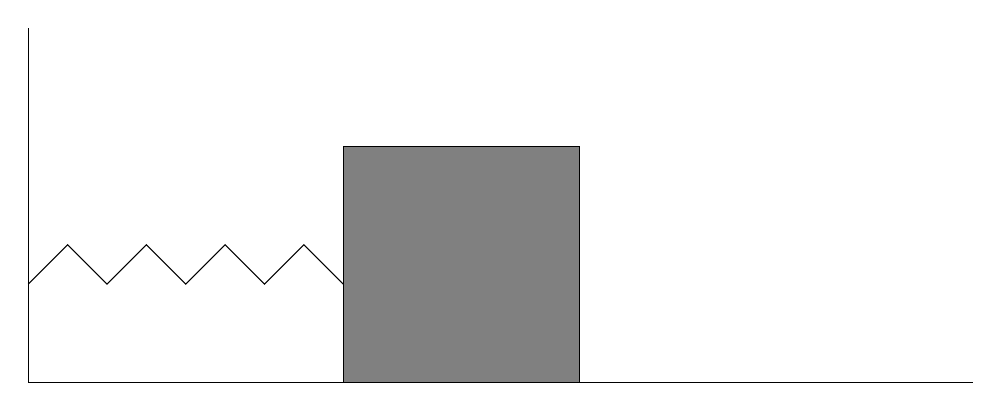
\begin{tikzpicture}
\draw (0,0) -- (12,0);
\draw (0,4.5) -- (0,0);
\filldraw[fill=gray] (4,3) -- (4,0) -- (7,0) -- (7,3) -- (4,3);
\draw (4,1.25) -- (3.5,1.75) -- (3,1.25) -- (2.5,1.75) -- (2,1.25) -- (1.5,1.75) -- (1, 1.25) -- (0.5,1.75) -- (0,1.25);
\end{tikzpicture}
\begin{center}
(Figure 7.4.1)
\end{center}
\
We will now begin discussing something that occurs very frequently not only in elementary physics but in more advanced physics. Often complex systems can be modeled using a system of simple harmonic systems. For example, we can model atom-atom interactions in solids as being a giant set of balls with strings attached between them approximating the force between the atoms. However, before we get there, we will consider the simple case of a spring pushing a mass m along a frictionless table as seen in Fig. 7.4.1. 


In these problems, we almost always take the approximation that the spring is massless. We can define a point called equilibrium at which, if not perturbed, the spring will not contract or expand. We can also assume that the spring enacts a linear restoring force upon the mass. This means that the force that the spring enacts is either pushing or pulling to the mass is proportional to the distance the mass is from equilibrium. We call the distance that the mass is away from equilibrium $x$ and we call the constant of proportionality between the distance and the true force $k$. It is important to recognize that the factor $k$ depends not on the mass, but on the spring itself. A more stiff string will be less happy to tolerate deviations away from its natural length, and therefore the restoring force will be greater. Meanwhile, a less stiff string will be more happy with deviations, and the restoring force will decrease. Because $k$ is proportional to the restoring force, it must be greater for more stiff strings and smaller for less stiff strings. 
We now know the magnitude of the restoring force, but we need to think of its direction. If you think about extending a string beyond its natural length while keeping one end fixed, there is going to be a force in the direction opposite to the direction of extension. Likewise, if we contract the spring, there is going to be a force in the direction opposite to how we contracted the spring. For this reason, we take the restoring force $F_{elastic}$ to be equal to $-kx$. Armed with this formula, we can use Newton’s second law to find the equation of motion for a mass $M$ that is moving with a string. We imagine that the string was displaced from the equilibrium at a distance $A$, where $A$ is the amplitude. We write that $ma=-kx$ as no other forces are involved in describing the motion of the system. We note that if $x=0$, then the acceleration is 0 and the system should not move. Simply moving the -$kx$ term to the other side and dividing both sides my m we find that \begin{equation}a+x\left(\frac{k}{m}\right)=0\end{equation}
We note that $a$ is just the second time derivative of $x$. We notice that because $k$ and $m$ are both positive, $a$ and $x$ must be of the reverse sign. Additionally, $a$ has to be equal to a constant multiple of $x$. Using these facts we can think about a function of $x$ with respect to $t$ that might satisfy these constraints. A polynomial won’t work because the second derivative of a polynomial is not a constant multiple of the original polynomial. Neither will an exponential because the second derivative of an exponential will be of the same sign as the original polynomial. However, a trigonometric function will work. The second derivative of $$a\cos\left(kx\right)$$ with respect to $x$ is simply $$-ak^2\cos\left(kx\right)$$ So if we take $x$ to be equal to $$A\cos\left(\omega t \right)$$ we find that $$-A\omega^2\cos\left(\omega t \right)+A\left(\frac{k}{m}\right)\cos\left(\omega t \right)=0$$ If we solve this equation, we find that $\omega$ is equal to $$\sqrt{\frac{k}{m}}$$ So our expression for $x$ is currently $$A\cos\left(\sqrt{\frac{k}{m}}t\right)$$ We assumed that at $t = 0$, and that the mass was displaced from equilibrium by a distance equal to the amplitude, so $x\left(0\right)$ must be equal to $A$. So in our expression, $A$ is the amplitude of oscillation. One thing we notice is that $x$ can never be greater than $A$ or less than $-A$ because a cosine function never is greater than 1 or less than -1. We can also note that the period of oscillation is equal to $$\frac{2\pi}{\omega}$$ The period of oscillation is the time it takes the spring to get back to the point where it originally was after leaving that point. This is just a general property of trigonometric functions that is best for you to discover on your own.  The frequency of oscillations is one divided by the period and is simply the number of complete oscillations that the system completes every 1 second. If you are not convinced, I challenge you to think a bit more about this point as it can be confusing at first. 
Now that we have derived the equation of motion for a horizontally moving mass and spring system, I challenge you to do the same thing for a similar system that is oscillating vertically. You can make a similar equation to the differential equation I have made before and attempt to solve it, but this will prove very difficult unless you have taken a course in differential equations. However, what you can do is imagine that the equilibrium is at the point at which the gravitational force acting on the mass is equal to the spring force acting on the box. We can take this point as being equal to 0, and then we have a normal mass-spring system. I challenge you to work out the specifics using both methods to see why the second one is much preferable.  

We have worked out the equation of motion for this string using Newton’s laws, but as we saw with other problems in Newtonian dynamics, we can formulate this problem in terms of energy. We will say that the potential energy of the system plus the kinetic energy of the system is constant because no work is being done on the system.  We will analyze the same system as above. The kinetic energy of the system is equal to $\frac{mv^2}{2}$ where $v$ is the velocity of the mass. The potential energy we can find by integrating the force that the spring does on the mass. Upon integrating, we find that the potential energy of the spring is equal to $\frac{-kx^2}{2}$, where $x$ is the distance displaced from equilibrium. With these two terms, we find that $$\frac{mv^2}{2}+\frac{kx^2}{2}$$ is a constant. This means that when one term is at the maximum, the other must be at a minimum. We can also find this by using the equation of motion in terms of sines and cosines we found above. The velocity will be 0 when the distance displaced is highest and vice versa. If you are not convinced by my work, I recommend you watch a good Walter Lewin video where he describes this topic. He also shows some demos that may help convince you that simple harmonic oscillation can be described using just sines and cosines. 